The goal of this project is to analyze two datasets providing different kinds of information about movies, TV shows, and other forms of visual entertainment.

In the following section, we'll focus on the tabular dataset, while the overview about the time series dataset composition and preparation can be found in Section \ref{time_series_analysis}.

This dataset is an extension of the one proposed in DM1: the records include key information about titles, insights into critical aspects such as awards and reviews, as well as ratings and further data about the title's production.

\subsection{Data Semantics, Duplicates and Train/Test Split}

The tabular dataset contains 149,531 records and 32 attributes; the nine attributes that were added to the original set from the DM1 dataset are reported in Tab. {\ref{tab:original_feats}}. This makes a total of nine categorical attributes, three binary attributes and 20 numerical attributes. Among the latter, only \textit{runtimeMinutes} and \textit{averageRating} can be classified as continuous, as the others mostly represent counts.

A first data quality check revealed only ten genuine duplicates, i.e. records sharing all feature values, which we dropped.

We then split the dataset, reserving 70\% for training, and the remaining 30\% for testing. As to avoid data leakage, we performed all subsequent data exploration exclusively on the training set. At the end of the data preparation stage, we applied all transformation and cleaning steps to the test set as well.

\begin{table*}
    \centering
    \renewcommand{\arraystretch}{1.2}
    \scriptsize
    \rowcolors{2}{}{gray!25}
    \begin{tabular}{p{3cm}p{7.5cm}p{3cm}}
        \toprule
        \textbf{Feature} & \textbf{Description} & \textbf{Type} \\ \midrule
        castNumber & Total Number of Cast individuals present within the IMDb title page. & Discrete. Ratio-scaled. \\
        companiesNumber & Total Number of companies that worked for the title. & Discrete. Ratio-scaled. \\
        regions & The regions for this version of the title. Some titles can belong to more than one class. & Categorical. 171 unique classes. \\
        averageRating & Weighted average of all the individual user ratings. & Continuous. Ratio-scaled. \\
        externalLinks & Total Number of External Links the title has within the IMDb page. & Discrete. Ratio-scaled. \\
        quotesTotal & Total Number of quotes the title has within the IMDb page. & Discrete. Ratio-scaled. \\
        writerCredits & Total number of writer credits of the title. & Discrete. Ratio-scaled. \\
        directorCredits & Total number of director credits of the title. & Discrete. Ratio-scaled. \\
        soundMixes & Technical specification of the sound mixes available for the title. Some titles can belong to more than one class. & Categorical. 59 unique classes. \\
        \bottomrule
    \end{tabular}
    \caption{New features in the extended dataset.}
    \label{tab:original_feats}
\end{table*}

\subsection{First Global Exploration of the Training Set}
A first global analysis of the dataframe's summary and descriptive statistics revealed missing values for \textit{endYear} (100,729), \textit{runtimeMinutes} (28,185), \textit{countryOfOrigin} (27,961) and \textit{genres} (1,887). Since most records are missing an \textit{endYear}, and the feature is strongly correlated to \textit{startYear}, we dropped it.

Since a great majority of records had no information about sound mixes, we decided to drop this feature as well.

\textit{bestRating}, \textit{worstRating}, and \textit{isRatable} were once again confirmed to be uninformative, as they only take one value for all records (10, 1, and 1, respectively), and were therefore dropped. We also dropped \textit{ratingCount}, as it was strongly correlated to \textit{numVotes}, and \textit{isAdult}, because it's redundant w.r.t. the \textit{adult} category in \textit{genres}.

Checking the values for the only remaining original binary attribute, \textit{canHaveEpisodes}, we noticed that only two records with a \textit{titleType} different from \textit{tvSeries} and \textit{tvMiniSeries} have a positive value. We corrected them: the first had been registered as a \textit{tvMovie} instead of \textit{tvSeries}, while the second was a short with no episodes.

Lastly, we removed the string \texttt{'\textbackslash \textbackslash N'}, which was prepended to all lists of \textit{regions}, making the feature consistent with \textit{numRegions}.


\subsection{Distribution of Categorical Variables and Statistics}

\begin{figure}
    \centering
    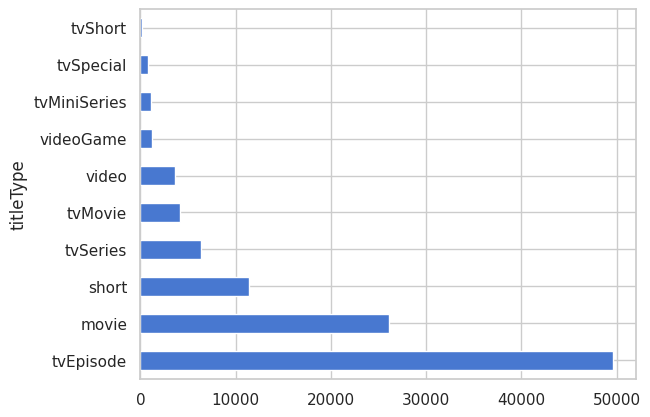
\includegraphics[width=\columnwidth]{../results/images/titleType_distribution.png}
    \caption{Distribution of \textit{titleTypes}.}
    \label{fig:titleType_distribution}
\end{figure}

\begin{figure}
    \centering
    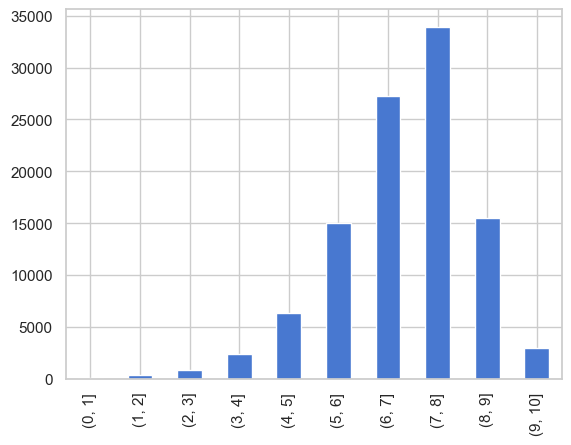
\includegraphics[width=\columnwidth]{../results/images/rating_distribution.png}
    \caption{Barplot for \textit{rating}.}
    \label{fig:rating_histogram.png}
\end{figure}

In this subsection, we studied the univariate and bivariate distribution of categorical variables, which all turned out to be unbalanced.

Differently from the DM1 dataset, the most popular \textit{\textbf{titleType}} is \textit{tvEpisode} (47\% of the records), followed by \textit{movie} (25\%) and \textit{short} (11\%); \textit{tvSpecial} (0.79\%) and \textit{tvShort} (0.17\%) are the classes with the lowest support (cf Fig \ref{fig:titleType_distribution}). With regard to \textit{\textbf{genres}}, the two most popular classes are by far \textit{Drama} and \textit{Comedy}, although it depends on \textit{titleType}.
Binned \textit{\textbf{rating}} follows a left-skewed distribution, with the mode being the [7,8) class (Fig. \ref{fig:rating_histogram.png}).
The most popular \textit{\textbf{countryOfOrigin}} and \textit{\textbf{region}} is the US, but both features have a substantial amount of missing values: \textit{nan} is the second most popular value for both.

We dropped \textit{soundMixes}: not only are most of its 59 unique values very rare, it has too many missing values to provide useful information.


\subsection{Distribution of Numeric Variables and Statistics}
\label{numeric_vars_analysis}
Before analyzing numeric variables, we added the same features we had added to the DM1 dataset:
\begin{itemize}
    \item \textit{numCountriesOfOrigin}: the number of countries listed for the record for the variable \textit{countryOfOrigin}. For the training set, the values range from 1 to 10.
    \item \textit{numGenres}: the number of genres listed in \textit{genres}. For the training set, the values range from 1 to 3.
    \item \textit{reviewsTotal}: the sum of \textit{criticReviewsTotal} and \textit{userReviewsTotal}.
    \item \textit{criticReviewsRatio}: the proportion of review from critics (\textit{criticsReviewTotal}) on the total number of reviews of a record (\textit{reviewsTotal}). For unreviewed records, it is set to zero.
    \item \textit{awardsAndNominations}: the sum of \textit{awardWins} and \textit{awardNominationsExcludeWins}.
\end{itemize}

A pairplot of all numeric variables, with KDE graphs on the diagonal, allowed us to gain a global view of both the features' univariate distribution and their pairwise correlations. Given the size of the dataset, we resorted to using a random sample of 20,000 records.
The great majority of the variables has a right-skewed distribution (\textit{writerCredits, numRegions, awardWins, totalImages, criticReviewsTotal, runtimeMinutes, userReviewsTotal, totalCredits, totalVideos, castNumber, numVotes, quotesTotal, awardNominationsExcludeWins, companiesNumber, externalLinks, awardsAndNominations, numCountriesOfOrigin, reviewsTotal}).
\textit{averageRating}, of course, follows the same left-skewed distribution observed for its discretized version, \textit{rating} (cf. Fig. \ref{fig:rating_histogram.png}).

We observed that some records have an implausibly long runtime, probably due to the inconsistent strategy adopted for the computation of the runtime for serialized content, for which sometimes the total runtime of a series is registered, rather than the average episode runtime.
In order to avoid this problem, we removed the runtime of all \textit{tvSeries}, \textit{tvMiniSeries}, and \textit{tvEpisodes} for which the value exceeded the 3rd quartile + 1.5 interquartile range for its specific category (105, 382.5 and 84 minutes, respectively); a total of 1560 records in the training set were affected.

A similar problem was found for \textit{writerCredits}: records with suspiciously high values are likely TV episodes for which all writers of the entire TV series were erroneously credited.
Therefore, we decided to remove the values for \textit{writerCredits} from 2100 \textit{tvEpisodes}, as they exceeded the 3rd quartile + 1.5 interquartile range (8.5 credits).

\subsection{Variable Transformation, Pairwise Correlations and Elimination of Variables}
We log-transformed all right-skewed variables, and used the Shapiro-Wilk test to determine whether they now resembled a normal distribution. None of them did, therefore we used Spearman's correlation coefficient in our correlation analysis.

% \begin{figure}
%     \centering
%     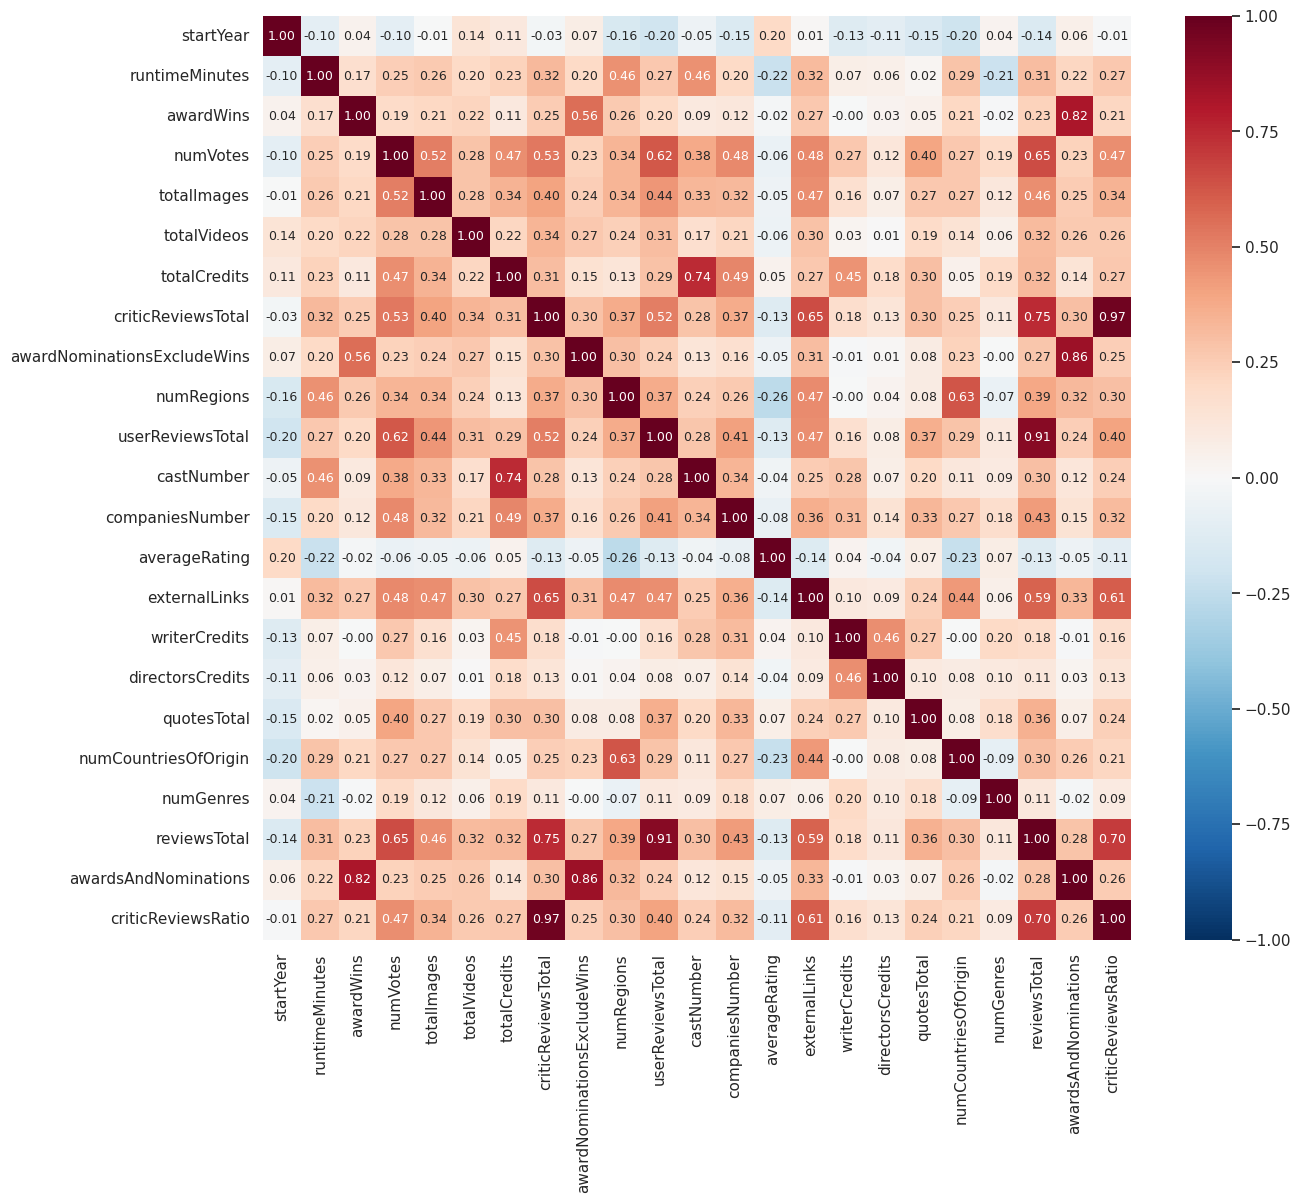
\includegraphics[width=\columnwidth]{../results/images/corr_heatmap_before.png}
%     \caption{Correlation heatmap before attribute removal.}
%     \label{fig:corr_heatmap_before.png}
% \end{figure}

We removed the following features because they were highly correlated to another feature: \textit{awardNominationsExcludeWins} (0.86, correlated with \textit{awardsAndNominations}), \textit{castNumber} (0.74, with \textit{totalCredits}).
Since all features regarding reviews and \textit{numVotes} were highly correlated with each other, we dropped them all with the exception of \textit{numVotes}, which has the least skewed distribution, and \textit{criticReviewsRatio}, which offer insights of a different nature. We however decided to conserve information about the presence/absence of reviews by users and critics with the creation of two new boolean features: \textit{hasUserReviews} and \textit{hasCriticsReviews}.

Moreover, we binarized features which overwhelmingly took on the value 0 (or 1, in the case of \textit{numCountriesOfOrigin} and \textit{directorsCredits}). The results of these transformations are reported in Table \ref{tab:binarized_features}.

\begin{table}
    \centering
    \small
    \setlength{\tabcolsep}{6pt}
    \renewcommand{\arraystretch}{1.1}
    \rowcolors{2}{}{gray!25}
    \begin{tabular}{l l c}
    \toprule
    \textbf{Original feature} & \textbf{Boolean version} & \textbf{\% True} \\
    \midrule
    awardWins            & hasAwards                       & 8.16  \\
    \makecell[l]{awardsAnd \\ Nominations}
                         & \makecell[l]{hasAwardsOr \\ Nominations} & 12.25 \\
    totalVideos          & hasVideos                       & 7.93  \\
    criticReviewsTotal   & hasCriticsReviews               & 24.88 \\
    userReviewsTotal     & hasUserReviews                  & 36.98 \\
    \makecell[l]{directors \\ Credits}
                         & \makecell[l]{moreDirectors \\ Credits} & 9.89  \\
    quotesTotal          & hasQuotes                       & 13.86 \\
    \makecell[l]{numCountries \\ OfOrigin}
                         & \makecell[l]{moreCountries \\ OfOrigin} & 5.05  \\
    \bottomrule
    \end{tabular}
    \caption{Binarization of numeric features.}
    \label{tab:binarized_features}
\end{table}


The total number of final features is 27; they are listed in Tables \ref{tab:dataset_numeric} and \ref{tab:dataset_categorical}. Among the remaining numeric features, the heatmap in Fig. \ref{fig:corr_heatmap_after.png} shows that \textit{externalLinks} exhibits a moderate to high positive correlation with \textit{criticReviewsRatio} (0.61) and a low to moderate correlation with \textit{numRegions}, \textit{numVotes} and \textit{totalImages} (around 0.47), while \textit{numVotes} is also mildly correlated to \textit{totalImages}, \textit{totalCredits}, \textit{criticReviewsRatio}, and \textit{companiesNumber} (between 0.47 and 0.52).

\begin{figure}
    \centering
    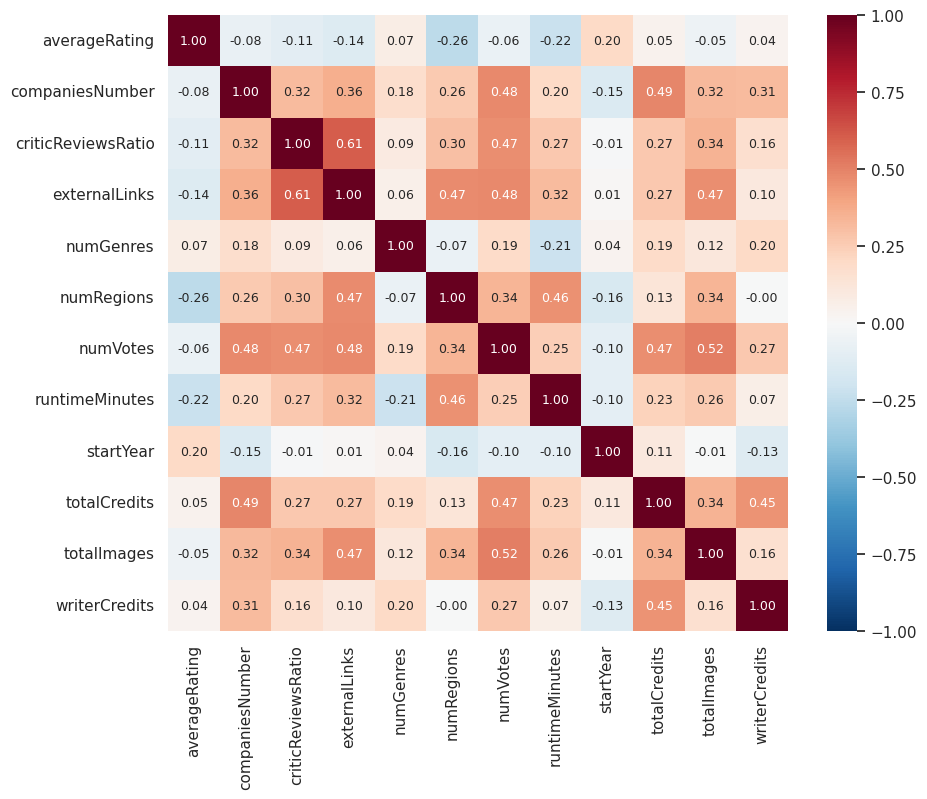
\includegraphics[width=\columnwidth]{../results/images/corr_heatmap_after.png}
    \caption{Correlation heatmap after attribute removal.}
    \label{fig:corr_heatmap_after.png}
\end{figure}


\begin{table*}[t]
    \centering
    \renewcommand{\arraystretch}{1.2}
    \scriptsize
    \rowcolors{2}{}{gray!25}
    \begin{tabular}{p{2.5cm}p{7cm}p{4.5cm}}
    \toprule
    \textbf{Feature} & \textbf{Description} & \textbf{Type} \\
    \midrule
    runtimeMinutes & Primary runtime of the title, in minutes. & Continuous. Ratio-scaled. \\
    startYear & Represents the release year of a title. In the case of TV Series, it is the series’ start year. & Discrete. Interval. \\
    numVotes & Number of votes the title has received. & Discrete. Ratio-scaled. Log-transformed. \\
    numRegions & The regions number for this version of the title. & Discrete. Ratio-scaled. Log-transformed. \\
    totalImages & Total number of images for the title within the IMDb title page. & Discrete. Ratio-scaled. Log-transformed. \\
    totalCredits & Total number of credits for the title. & Discrete. Ratio-scaled. Log-transformed. \\
    criticReviewsRatio & The proportion of reviews from critics on the total number of reviews of a record. For unreviewed records, it is set to 0. & Continuous. Ratio-scaled. \\
    numGenres & The number of genres listed for the variable \textit{genres}. & Discrete. Ratio-scaled. \\
    companiesNumber & Total number of companies that worked for the title. & Discrete. Ratio-scaled. \\
    externalLinks & Total number of external links the title has within the IMDb page. & Discrete. Ratio-scaled. \\
    writerCredits & Total number of writer credits of the title. & Discrete. Ratio-scaled. \\
    averageRating & Weighted average of all the individual user ratings. & Continuous. Ratio-scaled. \\
    \bottomrule
    \end{tabular}
    \caption{Numeric attributes after data preparation.}
    \label{tab:dataset_numeric}
\end{table*}

\begin{table*}[t]
    \centering
    \renewcommand{\arraystretch}{1.2}
    \scriptsize
    \rowcolors{2}{}{gray!25}
    \begin{tabular}{p{2.5cm}p{7cm}p{4.5cm}}
    \toprule
    \textbf{Feature} & \textbf{Description} & \textbf{Type} \\ \midrule
    originalTitle & Original title, in the original language. & Categorical; mostly unique classes (i.e. names). \\
    titleType & The type/format of the title (e.g. movie, short, tvseries, tvepisode, video, etc.). & Categorical, 10 classes. \\
    countryOfOrigin & The country where the title was primarily produced. & Categorical, 153 classes. Some titles can belong to more than 1 class. \\
    genres & The genre(s) associated with the title (e.g., drama, comedy, action). & Categorical, 29 classes. Some titles can belong to more than 1 class. \\
    regions & The regions for this version of the title. & Categorical, 171 unique classes. Some titles can belong to more than 1 class. \\
    rating & IMDB title rating class. & Ordinal, 10 values. \\
    hasAwards & Whether the title has won at least an award & Asymmetric binary. \\
    hasAwardsOrNominations & Whether the title was at least nominated for an award. & Asymmetric binary. \\
    canHaveEpisodes & Whether the title can have episodes. & Asymmetric binary. \\
    hasVideos & Whether the title IMDb title page has at least one video. & Asymmetric binary. \\
    moreCountriesOfOrigin & Whether the title was produced in more than one country. & Asymmetric binary. \\
    hasCriticsReviews & Whether the title has any critic reviews. & Asymmetric binary. \\
    hasUserReviews & Whether the title has any user reviews. & Asymmetric binary. \\
    moreDirectorsCredits & Whether the title has more than one director credits. & Asymmetric binary. \\
    hasQuotes & Whether the title has any quotes within the IMDb page. & Asymmetric binary. \\ \bottomrule
    \end{tabular}
    \caption{Categorical, ordinal, and binary attributes after data preparation.}
    \label{tab:dataset_categorical}
\end{table*}




\subsection{Handling Missing Values}
\label{handling_nan}
At this point, we still have missing values for \textit{countryOfOrigin}, \textit{region}, \textit{genres}, \textit{runtimeMinutes} and \textit{writerCredits}; some were preexisting, others were removed as detailed Subsec. \ref{numeric_vars_analysis}.
Since the distribution of \textit{runtimeMinutes} depends on \textit{titleType}, and the same holds true for \textit{writerCredits}, we imputed their missing values using the median value within each respective class.

On the other hand, we chose not to replace missing values for \textit{genres}, \textit{region} or \textit{countryOfOrigin}. They can easily be handled when performing the encoding for our methods without introducing bias, therefore we'd rather preserve the original distributions and correlations.


\subsection{Clustering}\label{sec:tabular_clustering}
\begin{figure*}
    \center
    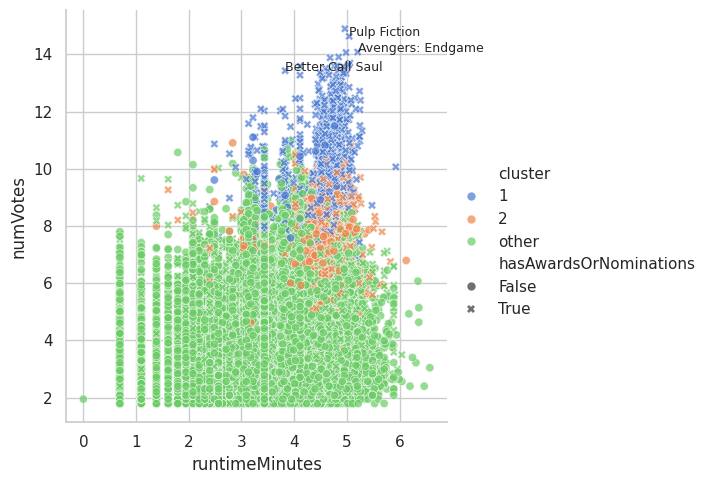
\includegraphics[width=.8\textwidth]{../results/images//understanding_clustering.png}
    \caption{Hierarchical clustering results on tabular data by runtime and number of votes.}
    \label{fig:tabular_clustering}
\end{figure*}

As part of the data understanding phase, we conducted hierarchical clustering on the dataset, using all numeric attributes.

Since the size of the dataset made it unfeasible to perform hierarchical clustering directly because of the computational cost of computing distances between all records, we firstly reduced our dataset to a more manageable 10,000 records, running k-means clustering with k=10,000.

We then performed hierarchical clustering on the centroids of K-Means clusters, experimenting with different linkage methods and inspecting the resulting dendrograms. We found that using average linkage yielded the most satisfactorily results. We then cut the dendrogram at an appropriate threshold and, after propagating cluster labels back to the entire dataset, analyzed the composition of the clusters.

We found 13 clusters of varying sizes, with the top cluster grouping one fifth of the entire dataset and the top four clusters grouping half of the dataset. Five clusters contained less than 5,000 records each.

For reasons that will become apparent in \ref{sec:anomaly_detection}, we concentrated our analysis on two smaller clusters: C1 (1,668 records) and C2 (3,923). These clusters belong to the same supercluster, that is merged latest of all with the rest of the dataset.

Both clusters are made up primarily from movies (with some tv series), and according to their distribution w.r.t. \emph{numVotes}, probably contain blockbuster movies and very popular TV series \ref{fig:tabular_clustering}.
In addition to that, almost 57\% of records from C1 received awards, a proportion that increases to 80\% when considering also nominations.
C2 records were also well received, with 45\% of them having received or being considered for awards.
In addition to that, 87\% of records from C1 and 45\% of records from C2 have videos on their IMDB page and almost all records from both C1 and C2 have both reviews from users and from critics.